% These slides have been made using the template found here: https://www.overleaf.com/latex/templates/beamer-presentation/zxrfltwmbcrt

\documentclass{beamer}
%
% Choose how your presentation looks.
%
% For more themes, color themes and font themes, see:
% http://deic.uab.es/~iblanes/beamer_gallery/index_by_theme.html
%
\mode<presentation>
{
  \usetheme{default}      % or try Darmstadt, Madrid, Warsaw, ...
  \usecolortheme{default} % or try albatross, beaver, crane, ...
  \usefonttheme{default}  % or try serif, structurebold, ...
  \setbeamertemplate{navigation symbols}{}
  \setbeamertemplate{caption}[numbered]
} 

\usepackage[english]{babel}
\usepackage[utf8x]{inputenc}
\usepackage{caption}

\begin{document}

\begin{frame}
% Example of title page for the projects carried out within DEDIS
% Copied from lasec 

% Simply include it in your mastex tex file: 
%        % Example of title page for the projects carried out within DEDIS
% Copied from lasec 

% Simply include it in your mastex tex file: 
%        % Example of title page for the projects carried out within DEDIS
% Copied from lasec 

% Simply include it in your mastex tex file: 
%        \input{cover}


% Updated October 2016


\newcommand{\logoepfl}[0]{
  \begin{center}
    
\includegraphics[width=4cm]{logo_epfl_coul.eps}
  \end{center}
  \vspace{0.3cm}
  \hrule
}
\newcommand{\project}[1]{
  \begin{center}
    \large{#1}
  \end{center}
  \vspace{1cm}
}
\newcommand{\department}[1]{
  \begin{center}
    \large{#1}
  \end{center}
}
\newcommand{\lab}[1]{
  \begin{center}
    \large{#1}
  \end{center}
}
\newcommand{\supervisor}[3]{
  \begin{center}
    \begin{normalsize}{
        \bf #1}\\#2\\#3
    \end{normalsize}
  \end{center}
}
\renewcommand{\author}[1]{
  \begin{center}
    \Large{#1}
  \end{center}
  \vspace{0.5cm}
}
\renewcommand{\title}[1]{
  \vspace{3cm}
  \begin{center}
    \huge{#1}
  \end{center}
  \vspace{1.7cm}
}
\renewcommand{\date}[2]{
  \begin{center}
    \normalsize{#1 #2}
  \end{center}
  \vspace{0.5cm}
}


\thispagestyle{empty}


% begin title page
  \logoepfl
  
  \title{Cross-Platform Mobile Application for the Cothority}
  
  \author{Cedric Maire}
  \department{School of Computer and Communication Sciences}
  \lab{Decentralized and Distributed Systems Lab}
  \project{Semester Project}
  
  \date{January}{2018}

  \begin{center}
    \begin{tabular}{cc}
      \begin{tabular}{p{4.0cm}}
        \supervisor{Responsible}{Prof. Bryan Ford}{EPFL / DeDiS}
      \end{tabular}&
      \begin{tabular}{p{4.0cm}}
        \supervisor{Supervisor}{Linus Gasser}{EPFL / DeDiS}
      \end{tabular}
    \end{tabular}
  \end{center}

% end title page



% Updated October 2016


\newcommand{\logoepfl}[0]{
  \begin{center}
    
\includegraphics[width=4cm]{logo_epfl_coul.eps}
  \end{center}
  \vspace{0.3cm}
  \hrule
}
\newcommand{\project}[1]{
  \begin{center}
    \large{#1}
  \end{center}
  \vspace{1cm}
}
\newcommand{\department}[1]{
  \begin{center}
    \large{#1}
  \end{center}
}
\newcommand{\lab}[1]{
  \begin{center}
    \large{#1}
  \end{center}
}
\newcommand{\supervisor}[3]{
  \begin{center}
    \begin{normalsize}{
        \bf #1}\\#2\\#3
    \end{normalsize}
  \end{center}
}
\renewcommand{\author}[1]{
  \begin{center}
    \Large{#1}
  \end{center}
  \vspace{0.5cm}
}
\renewcommand{\title}[1]{
  \vspace{3cm}
  \begin{center}
    \huge{#1}
  \end{center}
  \vspace{1.7cm}
}
\renewcommand{\date}[2]{
  \begin{center}
    \normalsize{#1 #2}
  \end{center}
  \vspace{0.5cm}
}


\thispagestyle{empty}


% begin title page
  \logoepfl
  
  \title{Cross-Platform Mobile Application for the Cothority}
  
  \author{Cedric Maire}
  \department{School of Computer and Communication Sciences}
  \lab{Decentralized and Distributed Systems Lab}
  \project{Semester Project}
  
  \date{January}{2018}

  \begin{center}
    \begin{tabular}{cc}
      \begin{tabular}{p{4.0cm}}
        \supervisor{Responsible}{Prof. Bryan Ford}{EPFL / DeDiS}
      \end{tabular}&
      \begin{tabular}{p{4.0cm}}
        \supervisor{Supervisor}{Linus Gasser}{EPFL / DeDiS}
      \end{tabular}
    \end{tabular}
  \end{center}

% end title page



% Updated October 2016


\newcommand{\logoepfl}[0]{
  \begin{center}
    
\includegraphics[width=4cm]{logo_epfl_coul.eps}
  \end{center}
  \vspace{0.3cm}
  \hrule
}
\newcommand{\project}[1]{
  \begin{center}
    \large{#1}
  \end{center}
  \vspace{1cm}
}
\newcommand{\department}[1]{
  \begin{center}
    \large{#1}
  \end{center}
}
\newcommand{\lab}[1]{
  \begin{center}
    \large{#1}
  \end{center}
}
\newcommand{\supervisor}[3]{
  \begin{center}
    \begin{normalsize}{
        \bf #1}\\#2\\#3
    \end{normalsize}
  \end{center}
}
\renewcommand{\author}[1]{
  \begin{center}
    \Large{#1}
  \end{center}
  \vspace{0.5cm}
}
\renewcommand{\title}[1]{
  \vspace{3cm}
  \begin{center}
    \huge{#1}
  \end{center}
  \vspace{1.7cm}
}
\renewcommand{\date}[2]{
  \begin{center}
    \normalsize{#1 #2}
  \end{center}
  \vspace{0.5cm}
}


\thispagestyle{empty}


% begin title page
  \logoepfl
  
  \title{Cross-Platform Mobile Application for the Cothority}
  
  \author{Cedric Maire}
  \department{School of Computer and Communication Sciences}
  \lab{Decentralized and Distributed Systems Lab}
  \project{Semester Project}
  
  \date{January}{2018}

  \begin{center}
    \begin{tabular}{cc}
      \begin{tabular}{p{4.0cm}}
        \supervisor{Responsible}{Prof. Bryan Ford}{EPFL / DeDiS}
      \end{tabular}&
      \begin{tabular}{p{4.0cm}}
        \supervisor{Supervisor}{Linus Gasser}{EPFL / DeDiS}
      \end{tabular}
    \end{tabular}
  \end{center}

% end title page

\end{frame}

\section{Cothority}
\begin{frame}{Cothority}

\begin{figure}[h]
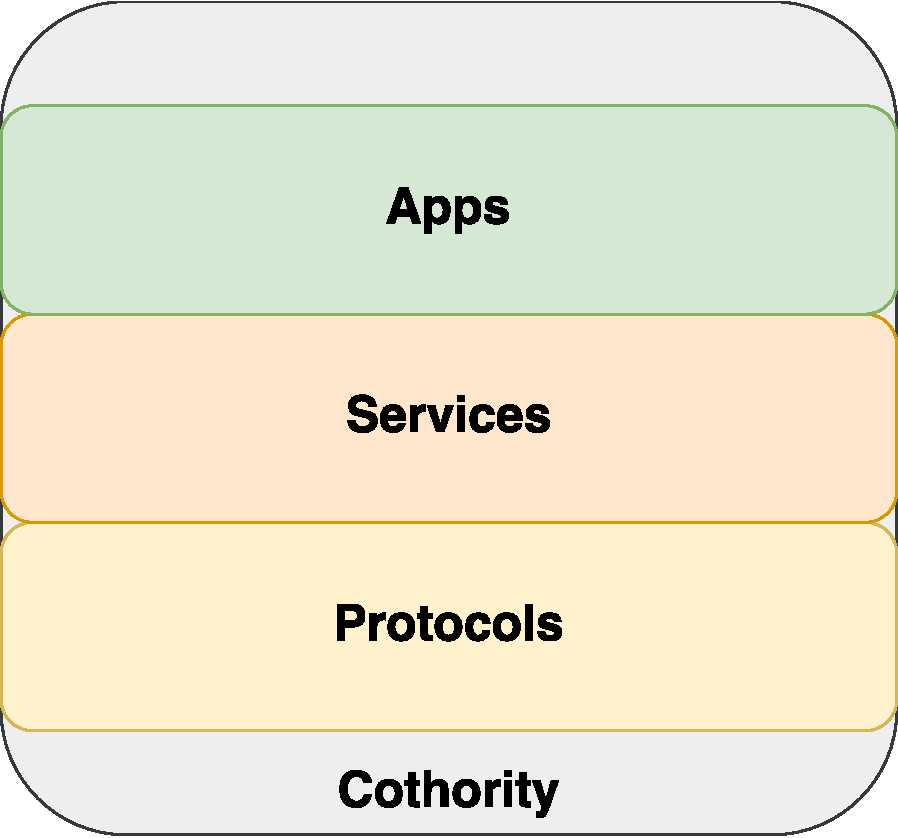
\includegraphics[scale=.5]{graphic/cothority.pdf}
\centering
\caption*{Cothority Framework}
\end{figure}

\end{frame}

\section{Why CPMAC?}
\begin{frame}{Why CPMAC?}

\begin{figure}[h]
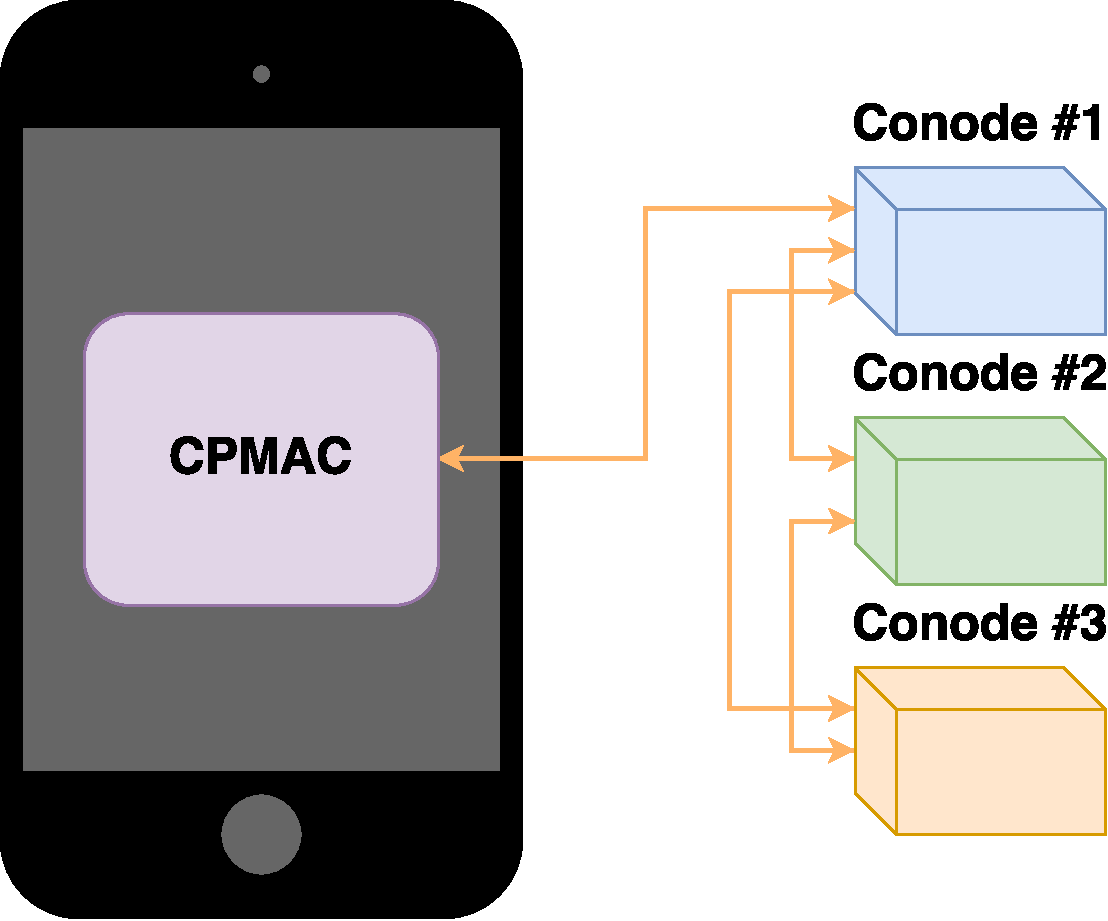
\includegraphics[scale=.45]{graphic/communication.pdf}
\centering
\caption*{Communication}
\end{figure}

\end{frame}

\section{CPMAC}
\begin{frame}{CPMAC}

\begin{figure}[h]
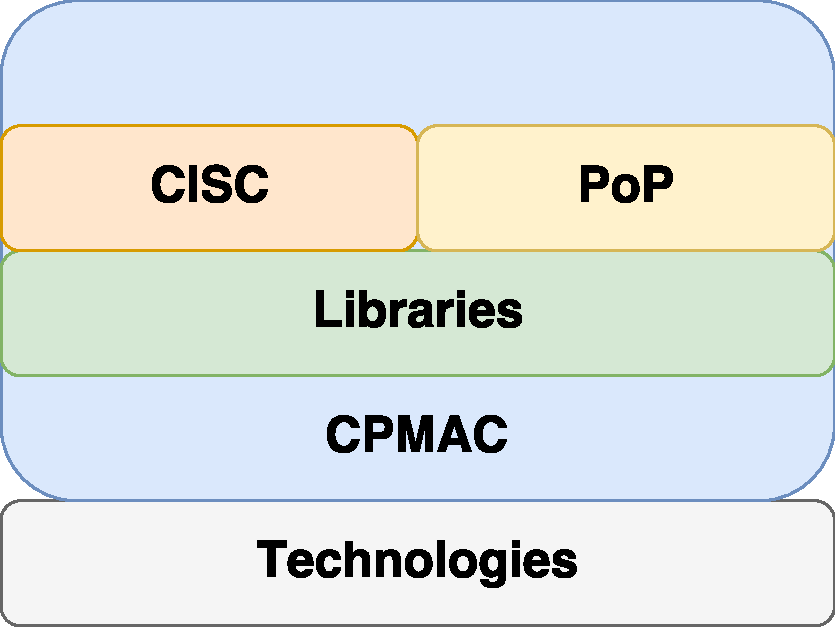
\includegraphics[scale=.6]{graphic/cpmac.pdf}
\centering
\caption*{CPMAC App}
\end{figure}

\end{frame}

\section{DeDjS}
\begin{frame}{DeDjS}

\begin{figure}[h]
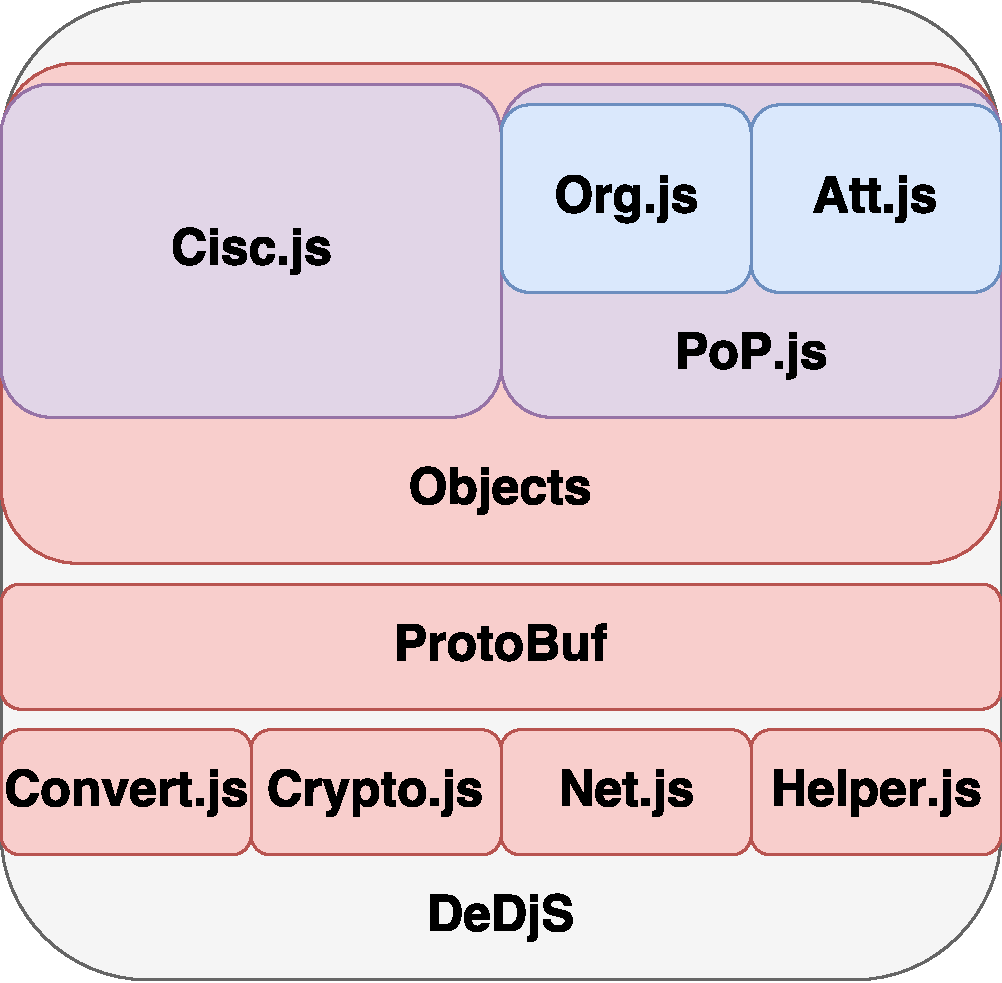
\includegraphics[scale=.4]{graphic/dedjs.pdf}
\centering
\caption*{DeDjS Library}
\end{figure}

\end{frame}

\end{document}

